\documentclass[tikz,border=2pt]{standalone}

\usepackage[T1]{fontenc}
\usepackage{xcolor}
\usetikzlibrary{arrows.meta,calc,shapes}

\definecolor{kvfourhundred}{HTML}{C62828}
\definecolor{kvtwohundredtwenty}{HTML}{1565A7}
\definecolor{kvonethirtytwo}{HTML}{2E8B57}
\definecolor{mapland}{HTML}{F2F0E8}
\definecolor{mapborder}{HTML}{6B7280}
\definecolor{mapgrid}{HTML}{CBD5E1}

\begin{document}
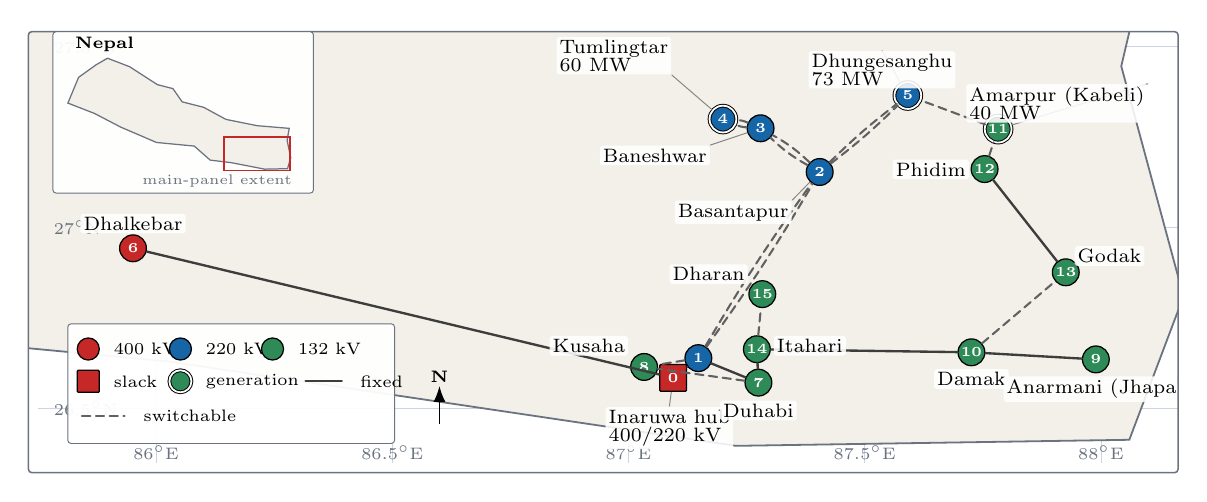
\begin{tikzpicture}[
  x=1cm,y=1cm,
  bus/.style={circle,draw=black,line width=0.45pt,minimum size=3.4mm,
    inner sep=0pt,font=\fontsize{5.4}{5.4}\selectfont\bfseries},
  bus400/.style={bus,fill=kvfourhundred,text=white},
  slack/.style={bus400,rectangle,rounded corners=0.35pt},
  bus220/.style={bus,fill=kvtwohundredtwenty,text=white},
  bus132/.style={bus,fill=kvonethirtytwo,text=white},
  generator/.style={double,double distance=0.65pt,line width=0.35pt},
  fixed/.style={draw=black!76,line width=0.85pt,line cap=round},
  switchable/.style={draw=black!62,line width=0.75pt,
    dash pattern=on 3pt off 2pt,line cap=round},
  leader/.style={draw=black!48,line width=0.35pt},
  maplabel/.style={font=\fontsize{6.6}{7.4}\selectfont,align=left,
    fill=white,fill opacity=0.88,text opacity=1,inner sep=1.1pt,
    rounded corners=0.7pt},
  gridlabel/.style={font=\fontsize{6}{6.5}\selectfont,text=mapborder},
  every node/.style={font=\scriptsize}
]

% Main-panel projection: x=6(lon-85.75), y=4.6(lat-26.35).
\begin{scope}
  \clip (-0.12,-0.12) rectangle (14.48,5.48);
  \fill[white] (-0.12,-0.12) rectangle (14.48,5.48);

  \foreach \x in {1.5,4.5,7.5,10.5,13.5}
    \draw[mapgrid,line width=0.25pt] (\x,0) -- (\x,5.48);
  \foreach \y in {0.69,2.99,5.29}
    \draw[mapgrid,line width=0.25pt] (0,\y) -- (14.48,\y);

  % Simplified Natural Earth outline of Nepal, cropped to the east.
  \path[fill=mapland,draw=mapborder,line width=0.65pt]
    (14.223,7.022) -- (13.759,5.041) -- (14.549,2.118) --
    (13.861,0.297) -- (8.865,0.220) -- (1.646,1.293) --
    (-2.989,1.731) -- (-6.450,4.071) -- (-14.675,4.667) --
    (-22.500,7.247) -- (-28.157,9.504) -- (-33.969,11.245) --
    (-31.640,15.547) -- (-27.832,17.634) -- (-25.345,18.734) --
    (-20.535,17.320) -- (-14.477,14.323) -- (-11.106,13.663) --
    (-9.093,11.454) -- (-4.430,10.547) -- (0.440,8.526) --
    (7.227,7.472) -- cycle;

  \node[gridlabel] at (1.5,0.14) {$86^{\circ}$E};
  \node[gridlabel] at (4.5,0.14) {$86.5^{\circ}$E};
  \node[gridlabel] at (7.5,0.14) {$87^{\circ}$E};
  \node[gridlabel] at (10.5,0.14) {$87.5^{\circ}$E};
  \node[gridlabel] at (13.5,0.14) {$88^{\circ}$E};
  \node[gridlabel,anchor=west] at (0.08,0.69) {$26.5^{\circ}$N};
  \node[gridlabel,anchor=west] at (0.08,2.99) {$27^{\circ}$N};
  \node[gridlabel,anchor=west] at (0.08,5.29) {$27.5^{\circ}$N};

  % WGS84 substation/settlement positions.  The co-located Inaruwa
  % voltage sections are separated slightly to expose the transformer.
  \coordinate (inaruwaGeo) at (8.228,1.209);
  \node[slack,xshift=-1.6mm,yshift=-1.25mm] (i400) at (inaruwaGeo) {0};
  \node[bus220,xshift=1.6mm,yshift=1.25mm] (i220) at (inaruwaGeo) {1};
  \node[bus400] (dhalkebar) at (1.208,2.729) {6};
  \node[bus220] (basantapur) at (9.929,3.698) {2};
  \node[bus220] (baneshwar) at (9.178,4.253) {3};
  \node[bus220,generator] (tumlingtar) at (8.700,4.370) {4};
  \node[bus220,generator] (dhungesanghu) at (11.048,4.669) {5};
  \node[bus132] (duhabi) at (9.151,1.023) {7};
  \node[bus132] (kusaha) at (7.699,1.222) {8};
  \node[bus132] (anarmani) at (13.436,1.318) {9};
  \node[bus132] (damak) at (11.856,1.408) {10};
  \node[bus132,generator] (amarpur) at (12.195,4.242) {11};
  \node[bus132] (phidim) at (12.023,3.735) {12};
  \node[bus132] (godak) at (13.054,2.424) {13};
  \node[bus132] (itahari) at (9.131,1.447) {14};
  \node[bus132] (dharan) at (9.200,2.147) {15};

  % Fixed transmission elements.
  \draw[fixed] (dhalkebar) -- (i400);
  \draw[fixed] (i400) -- (i220);
  \draw[fixed] (i220) -- (duhabi);
  \draw[fixed] (duhabi) -- (itahari);
  \draw[fixed] (itahari) -- (damak);
  \draw[fixed] (damak) -- (anarmani);
  \draw[fixed] (phidim) -- (godak);

  % Switchable Koshi-corridor double circuits.
  \draw[switchable] (i220) to[bend left=2.6] (basantapur);
  \draw[switchable] (i220) to[bend right=2.6] (basantapur);
  \draw[switchable] (basantapur) to[bend left=7] (baneshwar);
  \draw[switchable] (basantapur) to[bend right=7] (baneshwar);
  \draw[switchable] (baneshwar) to[bend left=10] (tumlingtar);
  \draw[switchable] (baneshwar) to[bend right=10] (tumlingtar);
  \draw[switchable] (basantapur) to[bend left=3.5] (dhungesanghu);
  \draw[switchable] (basantapur) to[bend right=3.5] (dhungesanghu);

  % Switchable 132 kV ties.
  \draw[switchable] (i220) -- (kusaha);
  \draw[switchable] (duhabi) -- (kusaha);
  \draw[switchable] (itahari) -- (dharan);
  \draw[switchable] (damak) -- (godak);
  \draw[switchable] (phidim) -- (amarpur);
  \draw[switchable] (amarpur) -- (dhungesanghu);

  % Labels and generation annotations.
  \node[maplabel,anchor=south] at (1.208,2.91) {Dhalkebar};
  \draw[leader] (i400) -- (8.02,0.72);
  \node[maplabel,anchor=north] at (8.02,0.72)
    {Inaruwa hub\\[-1pt]\scriptsize 400/220 kV};

  \draw[leader] (tumlingtar) -- (8.05,4.93);
  \node[maplabel,anchor=south east] at (8.05,4.93)
    {Tumlingtar\\[-1pt]\scriptsize 60 MW};
  \draw[leader] (baneshwar) -- (8.54,4.04);
  \node[maplabel,anchor=north east] at (8.54,4.04) {Baneshwar};
  \draw[leader] (basantapur) -- (9.58,3.34);
  \node[maplabel,anchor=north east] at (9.58,3.34) {Basantapur};
  \draw[leader] (dhungesanghu) -- (10.72,5.24);
  \node[maplabel,anchor=north] at (10.72,5.24)
    {Dhungesanghu\\[-1pt]\scriptsize 73 MW};

  \node[maplabel,anchor=north] at (9.15,0.80) {Duhabi};
  \node[maplabel,anchor=south east] at (7.50,1.36) {Kusaha};
  \node[maplabel,anchor=west] at (9.34,1.49) {Itahari};
  \node[maplabel,anchor=south east] at (9.02,2.27) {Dharan};
  \node[maplabel,anchor=north] at (11.856,1.20) {Damak};
  \node[maplabel,anchor=north] at (13.436,1.11) {Anarmani (Jhapa)};
  \node[maplabel,anchor=south west] at (13.16,2.50) {Godak};
  \node[maplabel,anchor=east] at (11.83,3.73) {Phidim};
  \draw[leader] (amarpur) -- (14.10,4.82);
  \node[maplabel,anchor=north east] at (14.10,4.82)
    {Amarpur (Kabeli)\\[-1pt]\scriptsize 40 MW};

  \draw[-{Latex[length=2.0mm]},line width=0.55pt]
    (5.10,0.50) -- (5.10,0.98);
  \node[font=\fontsize{6}{6}\selectfont\bfseries] at (5.10,1.10) {N};
\end{scope}

\draw[mapborder,line width=0.55pt,rounded corners=1.2pt]
  (-0.12,-0.12) rectangle (14.48,5.48);

% National locator inset.
\begin{scope}[shift={(0.35,3.70)}]
  \fill[white,opacity=0.94,rounded corners=1.2pt]
    (-0.16,-0.27) rectangle (3.15,1.78);
  \draw[mapborder,line width=0.35pt,rounded corners=1.2pt]
    (-0.16,-0.27) rectangle (3.15,1.78);
  \path[fill=mapland,draw=mapborder,line width=0.45pt]
    (2.842,0.552) -- (2.815,0.401) -- (2.861,0.179) --
    (2.821,0.040) -- (2.530,0.034) -- (2.109,0.116) --
    (1.838,0.149) -- (1.636,0.327) -- (1.156,0.373) --
    (0.700,0.569) -- (0.370,0.741) -- (0.031,0.873) --
    (0.167,1.200) -- (0.389,1.359) -- (0.534,1.443) --
    (0.815,1.335) -- (1.168,1.107) -- (1.365,1.057) --
    (1.482,0.889) -- (1.754,0.820) -- (2.038,0.666) --
    (2.434,0.586) -- cycle;
  \draw[kvfourhundred,line width=0.65pt]
    (2.013,0.018) rectangle (2.853,0.438);
  \node[font=\fontsize{6}{6.5}\selectfont\bfseries,anchor=west]
    at (0.00,1.62) {Nepal};
  \node[font=\fontsize{5.4}{6}\selectfont,text=mapborder,anchor=east]
    at (3.00,-0.12) {main-panel extent};
\end{scope}

% Legend in the geographically empty southwest.
\begin{scope}[shift={(0.38,0.25)}]
  \fill[white,opacity=0.95,rounded corners=1.2pt]
    (0,0) rectangle (4.15,1.52);
  \draw[mapborder,line width=0.35pt,rounded corners=1.2pt]
    (0,0) rectangle (4.15,1.52);

  \node[bus400,minimum size=2.8mm] at (0.26,1.20) {};
  \node[font=\fontsize{6}{6.5}\selectfont,anchor=west]
    at (0.46,1.20) {400 kV};
  \node[bus220,minimum size=2.8mm] at (1.43,1.20) {};
  \node[font=\fontsize{6}{6.5}\selectfont,anchor=west]
    at (1.63,1.20) {220 kV};
  \node[bus132,minimum size=2.8mm] at (2.60,1.20) {};
  \node[font=\fontsize{6}{6.5}\selectfont,anchor=west]
    at (2.80,1.20) {132 kV};

  \node[slack,minimum size=2.8mm] at (0.26,0.79) {};
  \node[font=\fontsize{6}{6.5}\selectfont,anchor=west]
    at (0.46,0.79) {slack};
  \node[bus132,generator,minimum size=2.8mm] at (1.43,0.79) {};
  \node[font=\fontsize{6}{6.5}\selectfont,anchor=west]
    at (1.63,0.79) {generation};
  \draw[fixed] (3.02,0.79) -- (3.48,0.79);
  \node[font=\fontsize{6}{6.5}\selectfont,anchor=west]
    at (3.59,0.79) {fixed};

  \draw[switchable] (0.18,0.35) -- (0.72,0.35);
  \node[font=\fontsize{6}{6.5}\selectfont,anchor=west]
    at (0.84,0.35) {switchable};
\end{scope}

\end{tikzpicture}
\end{document}